% !TeX root = ../thesis.tex
\chapter{背景知識}
Like this \cite{726791, baevski2020wav2vec} and fade out.

\section{背景知識}

\section{深層類神經網路}

\subsection{簡介}

深層類神經網路是 McColloh 在 1950 年提出的計算模型,其概念取法自連結主意學派,旨在用計算模型模擬生物神經連結的現象。類神經網路最基本的單元為一個神經元(neuron),來自 1960 年 Rosenblatt 提出的感知器(Perceptron)模型,旨在根據輸入訊號給出的線性分類器,其數學是可以表達成:

$ x = 3 $
\( y = 57 \)
\( z = 4 \)

Like these. 像這樣子 \\
ook

$y=\sigma(w^\top x + b) $

\begin{figure}
    \centering
    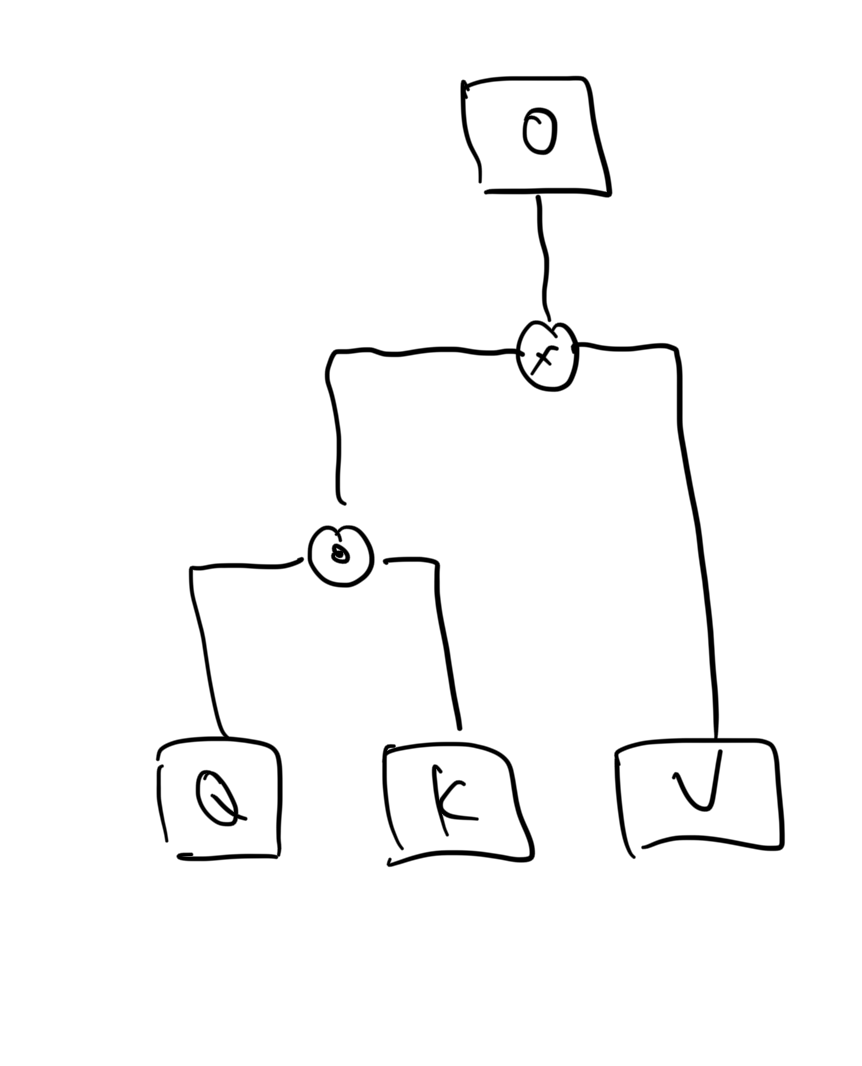
\includegraphics[width=0.5\linewidth]{figures/Yy.png}
    \caption{Enter Caption}
    \label{fig:enter-label}
\end{figure}

